\subsection{End-to-end generators fail under corridor multi-modality}
\paragraph{Fixed diagnostic cases (no cherry-picking).}
We first select diagnostic OD conditions with clear corridor-level multi-modality by auditing ground-truth routes (Sec.~\ref{sec:experiments}).
All qualitative overlays and collapse metrics are reported on these fixed cases.
In this draft, we focus on a representative Detroit case from WorldTrace \citep{opentrace_worldtrace}.

\paragraph{Averaging vs.\ interference.}
Figure~\ref{fig:mode-collapse} visualizes multiple samples for the same condition.
Deterministic L2 regression collapses to an overly direct ``mean'' route, consistent with destructive averaging under multi-modality.
An end-to-end diffusion generator avoids hard collapse, but in long-horizon generation its samples can become destination-inconsistent and diverge off-road, producing globally implausible trajectories.

\subsection{Hierarchical decomposition restores corridor diversity}
\paragraph{Corridor commitment from decision-stage sampling.}
When the decision stage explicitly samples a sparse waypoint skeleton, the generator recovers corridor-level alternatives.
This supports the hypothesis that corridor diversity must be represented as an explicit topological commitment rather than being left implicit in continuous coordinates.

\subsection{Commitment preservation is necessary for composition}
\paragraph{Naive composition can overwrite commitments.}
Composing a multi-modal decision sampler with a strong continuous executor can still lose corridor coverage: the execution stage may overwrite the committed corridor choice, collapsing the final routes into a single corridor even when the skeletons are diverse.
This shows that ``having a planner'' is not sufficient; the composition must preserve commitments.

\paragraph{Commitment-preserving refinement via residual scaling.}
Treating execution as a weak residual refinement (by scaling the execution residual) preserves corridor commitments while still refining local geometry.
This provides a controllable knob that balances corridor adherence against continuous-detail refinement and is a key practical ingredient in making the cascade work end-to-end.

\subsection{Data utility is stage-specific (design principle)}
\paragraph{Decision stage: semantics and map priors do not drive corridor commitment.}
We evaluate multiple inference-observable semantic representations for conditioning the decision stage, including endpoint covariates (POI density and land-use entropy), along-chord profiles, and OD-aligned grid encoders.
Across these settings, richer semantic representations provide limited and inconsistent benefit for corridor commitment.
Crucially, a matched-dimension random OD-keyed embedding yields comparable gains to weak endpoint semantics, indicating that apparent improvements are largely due to conditioning capacity rather than semantic content.
Moreover, injecting dense map priors into the decision stage can reduce corridor diversity and coverage (Table~\ref{tab:stage-specific}), reinforcing the view that corridor commitment is primarily topological.

\paragraph{Execution stage: soft road priors improve feasibility without accuracy loss.}
In contrast, applying OSM-derived feasibility priors at the execution stage yields a large and clean improvement.
Starting from the full-scale CascadeTraj outputs, a lightweight road-prior refinement improves the on-road rate from $0.91$ to $0.96$ without degrading best-of-$K$ ADE (Table~\ref{tab:stage-specific}).
This contrast---the same data source hurting decision but helping execution---provides actionable guidance on integrating heterogeneous urban data into hierarchical route generators.

\paragraph{Realistic route validation beyond scalar metrics.}
Figure~\ref{fig:realism} qualitatively and statistically validates realism.
On three fixed OD cases, our $K=20$ samples largely adhere to the road prior while maintaining diversity.
On the full split, our generated routes better match the ground-truth distributions of path length, detour factor (relative to straight-line distance; excluding degenerate near-zero chords), per-route on-road rate, and turn-angle statistics than end-to-end diffusion.

\begin{figure}[t]
  \centering
  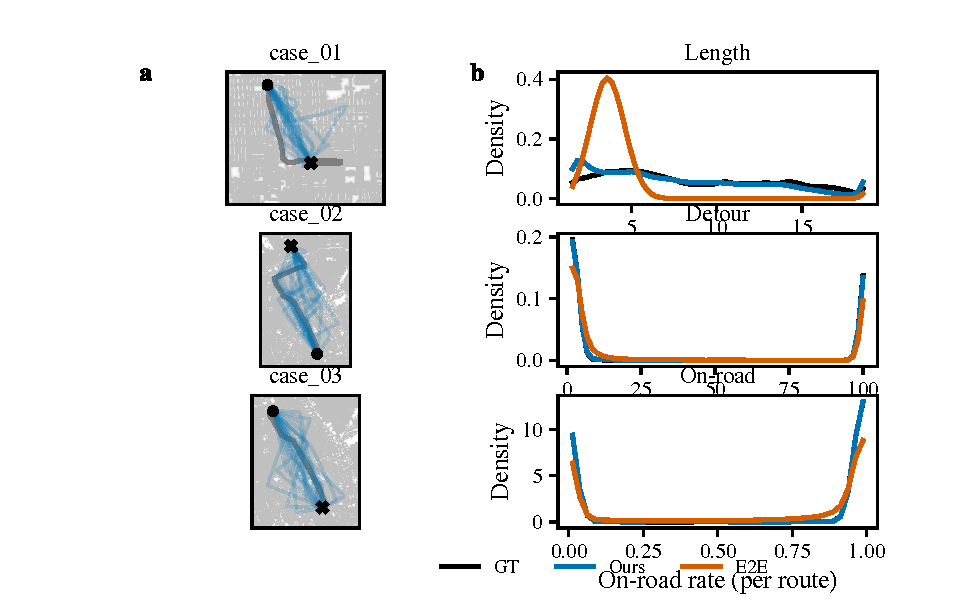
\includegraphics[width=\linewidth]{figures/fig_realism_validation.pdf}
  \caption{Realistic route generation validation (Detroit). \textbf{(a)} For three fixed OD cases, we overlay ground-truth routes (gray), $K=20$ samples from CascadeTraj (blue), and end-to-end diffusion (orange) on an OSM-derived road-probability basemap. \textbf{(b)} Distribution alignment for path length, detour factor (vs.\ straight-line distance; filtering near-zero chords), per-route on-road rate (fraction of points with road probability $\ge 0.5$), and turn-angle statistics.}
  \label{fig:realism}
\end{figure}

\subsection{Full-scale evaluation confirms the approach}
\paragraph{Beyond diagnostic cases.}
On the full Detroit benchmark split ($2295$ windows, $K=20$), CascadeTraj improves best-of-$K$ micro accuracy and feasibility over end-to-end diffusion (Table~\ref{tab:fullscale}).
In particular, CascadeTraj reduces best-of-$K$ ADE from $97.9$ to $23.8$ and increases the on-road rate from $0.83$ to $0.91$ (road-probability threshold $0.5$).
Because CascadeTraj enforces destination consistency via endpoint anchoring (Sec.~\ref{sec:endpoint-anchoring}), endpoint error (FDE) becomes less informative and we emphasize shape and feasibility metrics.

\paragraph{Interpreting global Jaccard diversity.}
On the full split, end-to-end diffusion exhibits higher occupancy-set Jaccard distance than CascadeTraj.
This does not necessarily indicate better corridor modeling: this proxy can be inflated by off-road wandering and mode interference that spreads samples across many grid cells.
We therefore interpret global Jaccard diversity jointly with feasibility and micro accuracy, and rely on corridor-level coverage metrics on fixed multi-modal cases to diagnose corridor commitment.

\begin{table}[t]
  \centering
  \small
  \begin{tabular}{lccc}
    \toprule
    Model & ADE$_{\text{best}}$ & On-road rate & Jaccard div. \\
    \midrule
    End-to-end Diffusion & 97.9 & 0.829 & 0.878 \\
    CascadeTraj (res$_{0.1}$) & 23.8 & 0.912 & 0.782 \\
    \bottomrule
  \end{tabular}
  \caption{Full-scale evaluation on Detroit (WorldTrace), $N=2295$ windows, $F=256$, $K=20$. ADE is best-of-$K$ in grid units. On-road rate uses OSM road probability threshold $0.5$. Jaccard diversity is the mean pairwise occupancy-set Jaccard distance (higher can be inflated by noisy off-road wandering).}
  \label{tab:fullscale}
\end{table}

\begin{table}[t]
  \centering
  \small
  \begin{tabular}{lccc}
    \toprule
    Variant & Cov / On-road & Div / road\_prob & JSD / ADE$_{best}$ \\
    \midrule
    \multicolumn{4}{l}{\textbf{Decision stage (E11, 5 diagnostic cases):} Cov$\uparrow$, Div$\uparrow$, JSD$\downarrow$} \\
    gridcnn (poi+entropy) & 1.000 & 0.928 & 0.013 \\
    gridcnn\_road (+road\_prob) & 0.904 & 0.763 & 0.032 \\
    \midrule
    \multicolumn{4}{l}{\textbf{Execution stage (E12, full-scale):} On-road$\uparrow$, road\_prob$\uparrow$, ADE$_{best}\downarrow$} \\
    baseline cascade & 0.912 & 0.894 & 23.8 \\
    +road prior (strong) & 0.964 & 0.958 & 23.8 \\
    \bottomrule
  \end{tabular}
  \caption{Stage-specific data utility. The same OSM-derived road signal harms decision-stage corridor modeling when used as conditioning (E11) but improves execution-stage feasibility when used as a soft refinement (E12).}
  \label{tab:stage-specific}
\end{table}
